\section{Introduction} \label{sec:intro}
Monitoring and modeling of large-scale stochastic phenomena with both spatial and temporal (spatiotemporal) evolution using a network of distributed sensors is a fundamental problem in many applications. Consider, for example, a team of robots with the task of destroying herbicide-resistant weeds on a farm (see Figure \ref{fig:cps}, also see ``\nameref{sb:ag}''). This team of robots needs to predict the weed growth across the whole farm  to make intelligent, coordinated decisions \cite{McAllistar18IROS}. However, the robots can only observe a limited part of the field at a time, leading to  the critical problem: how can a few robots that can only partially observe the field at any time predict the full state of the spatiotemporally-evolving weed growth over the entire field? The goal of this tutorial is to show the steps we have taken towards addressing this challenging problem. Examples of this kind of problem abound across many domains, including: modeling and monitoring of ocean heat content and acidification for oceanography using a network of satellites and surface sensors \cite{barnett2001detection}; prediction of traffic patterns using data from vehicles, cellphones, and traffic cameras; prediction of enemy movements through ground and aerial surveillance; and prediction of extreme weather events  using data from weather stations and aerial drones \cite{heaton2011spatio}. The rapid advances in the computational power of compact systems and robotics in general has led to an explosion of real-world applications for such distributed cyber-physical systems. % \cite{barnett2001detection}future seismicity \cite{bungum2005postglacial}, land use change in urbanization \cite{deng2009spatio}, and extreme weather events \cite{heaton2011spatio}. One emerging and compelling example is 
 
\begin{figure}[h] %{r}{0.5\textwidth}
	\centering
	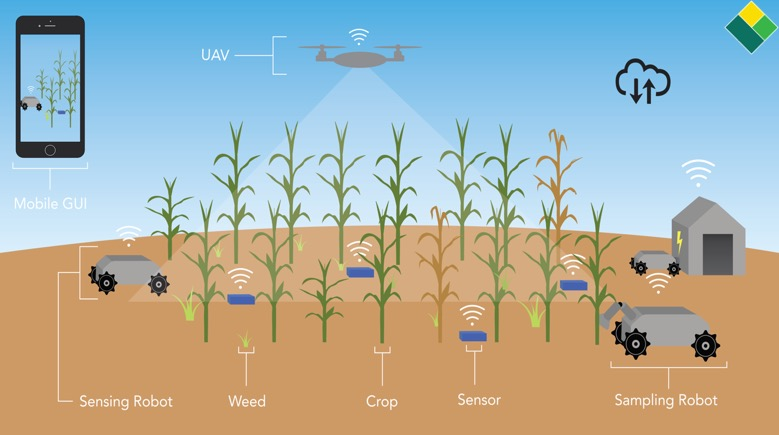
\includegraphics[width=\columnwidth]{agrobot_cps.jpg}
		\caption{A Cyber Physical system consisting of a distributed team of robots for mechanical weed management on a farm. Image courtesy EarthSense inc.}
	\label{fig:cps}
\end{figure}
%With rapid advances in low-cost data processing hardware and mobile robotics, large scale cyber physical systems capable of monitoring 

 %In situations where this is possible, such as in computational fluid dynamics, the resulting models may become computationally intractable, requiring hours or even days on supercomputers, and far out of the reach of compute and connectivity capabilities on robots or sensors deployed in the field.  On the other hand, recent advances in machine learning indicate that perhaps data-driven modeling could be a promising way  .  


%There has been significant interest in developing distributed modeling and monitoring algorithms for such systems, however, 


%The objective of this article is to introduce a modeling and monitoring mechanism that marries together recent successes of machine learning with powerful results from systems and control theory. We achieve this by demonstrating how critical properties such as observability and controllability can be derived systems can be embedded inside feature spaces of machine learning models We now elaborate the context behind this claim.  
% Let us dwell on this point a bit, its rather tempting to dismiss deep learning models and machine learning in general as blackboxes, but one can't argue with the success of those models. Taking a deeper look, one realizes that all machine learning is trying to do is to automatically learn a state-space (termed as the feature space cite our sidebar) which may be nonlinarly generated using other features. Infact sidebar blabla discusses three ways in which one could come up with these features, what the engineering community prefers is the features of the first kind which are physically directly relatable to physical quantities. 
%The success of machine learning in complex problems teaches us that giving up on 
% allows one to solve very tough problems. SO its not the feature space that's the problem, 
%When one gives up physical interpretability, it becomes rather  difficult to understand why something is broken, or what guarantees could be put in place to ensure performance remains within bounds. with the traditional deep learning models, the only real way of dealing with this right now is sampling based, that is through thousands of simulations. Going a step further, its difficult to come up with guarantees on certain behaviors of the model. Observability and controllability are two fundamental guaratnees that controls interpretable models have provided us. SO the question that we ask here is does embedding interpretable models in complex feature spaces allows us to recover some of those guarantees while leveraging the strength of feature learning.

%Taking a broader perspective, complex dynamical systems such as agriculture and weather are very difficult to model and control using traditional first principles based approaches alone. On the other hand


These types of applications need to estimate complex, stochastic dynamics that are distributed over space and time. The key constraint is the number of spatially distributed sensors available, which are not enough to entirely cover the whole space at any given moment in time. One approach to solving the problem under this constraint is to use a predictive model of the phenomenon which informs our sensing strategy. %It may be difficult to model such systems with spatiotemporal dynamics using first principles alone. 
While the modeling of such spatiotemporal phenomena has traditionally been the object of study in geostatistics, it has in recent years gained more attention in the machine learning community \cite{cressie2011statistics}. The data-driven models developed by machine learning techniques provide a way to capture complex spatiotemporal phenomena which are not easily modeled by first-principles alone. However, these models are limited by the data sets they are trained on, and the high variability of complex distributed physical systems makes it even more challenging. For example, a model trained over years of weed growth data in one field doesn't necessarily generalize to another, and a model trained on the past few years of data is still unreliable to predict weather variability in the following year. What is needed is not just a \textit{predict} system but a \textit{predict-and-correct} system. This tutorial shows how to design just such a system for these kind of problems. The system utilizes kernel methods for modeling, Bayesian filtering theory for prediction correction, and exploits the mathematical structure of the regression and dynamics models to place the sensors. 


 %, such as those described by stochastic partial differential equations with uncertain parameters. %, such as stochastic partial differential equations. 

In the machine learning community, kernel methods represent a class of well-studied and powerful methods for regression in spatial domains. In these techniques, correlations between the input variables are related via covariance kernels, and the model is generated by a linear combination of the kernels \cite{RasmussenWilliams2005,schoelkopf01kernelbased,scholkopf2002learning}. In recent years, kernel methods have been applied to spatiotemporal regression problems with varying degrees of success \cite{cressie2011statistics,RasmussenWilliams2005}. Many recent methods have focused on nonstationary covariance kernel design and algorithms for learning the associated hyperparameters \cite{garg2012AAAI,ma2003nonstationary,plagemann2008nonstationary,todescato2017efficient}. These methods, which focus on the careful design of covariance kernels, have been proposed as an alternative to the naive approach of simply including time as an additional input dimension in the kernel \cite{Chowdhary13_CDC1}. The careful design/optimization of a covariance kernel avoids an explosion in the number of parameters used by the model, which would be inevitable in the naive approach, and can better account for spatiotemporal couplings. Such covariance kernels, however, do not scale in the face of large-scale phenomena since the optimization of the kernel hyperparameters is non-convex and computationally demanding for large datasets \cite{sra2012optimization}. Deep learning also suffers from similar issues, and moreover lacks the spatial encoding properties of certain kernels, which are exploited by the strategy outlined in this tutorial.

% However, there are two key difficulties with existing kernel-based (and other) machine learning approaches for prediction over complex spatiotemporally-varying systems. The first is the scalability of the model to large scale phenomena, which manifests due to the general non-convexity of the problem of optimizing the covariance kernel (known as hyperparameter optimization), leading to methods that are difficult to implement, susceptible to getting stuck at local minima, and computationally demanding for large datasets \cite{sra2012optimization}. This has also been a key issue in for deep learning models with this problem. % \cite{sra2012optimization}. 

%The second key difficulty is that 

No matter how much data the model is trained on, it cannot completely capture the variability of real-world systems with complex spatiotemporal dynamics. This is a problem that the controls community is quite aware of; their solution to this is built upon feedback, leading to fundamental notions of observability and controllability which can be used to build robust state estimators and controllers. To bring these ideas to fruition in the spatiotemporal problem, we needed a way to find where sensing/control should be performed to ensure that the state estimation problem can be made observable/controllable. % Current ML models do not provide such insight. In particular, 
%\rr{
While methods such as \cite{todescato2017efficient} have succeeded in using nonstationary kernels that evolve efficiently using feedback, it is not clear how notions of observability and controllability could be utilized with it or other existing kernel-based machine learning models, and how observers and controllers can be embedded within such models.
%} % for the large scale spatiotemporal phenoemena. }
Computational challenges can be addressed with faster methods or increasing computational power; however, addressing the latter, more fundamental challenge in designing robust observers/controllers is particularly important in the design of reliable engineering systems, such as distributed sensor/actuator networks intended for monitoring physical phenomena, autonomous soft-robots, or other physical systems with distributed sensing and actuation.  %Consider in specific the problem of designing an optimal distributed sensor network for ``monitoring'' a spatiotemporally evolving function. 
%Some of the fundamental engineering questions that are of importance here are Given an approximate predictive model of the spatiotemporal phenomena, how can the current latent state of the phenomena be estimated using as few sensor measurements as possible?  
% 
 % and are left for exploration in future work.  
   
%In addition to the challenge of modeling spatiotemporally varying processes, we are interested in addressing the second very important, and widely unaddressed challenge:

%To focus the development of the theory, we posit the challenging problem of ``monitoring'' a spatiotemporal phenoemena: Given an approximate predictive model of the spatiotemporal phenomena, how can the current latent state of the phenomena be estimated using as few sensor measurements as possible? This is called the \emph{monitoring problem}. Monitoring a spatiotemporal phenomenon is concerned with estimating its current state, predicting its future evolution, and inferring the initial conditions utilizing limited sensor measurements. The key challenges here manifest due to the fact that it is typically infeasible or expensive to deploy sensors at a large scale across vast spatial domains. %For example, in monitoring the flux of $CO_2$ over underground $CO_2$ storage sites, the number of sensors and sensing locations are limited due to cost or geography. %In another example, when monitoring the state of dynamically evolving enemy deployment over a contested area, the availability of measurements is limited due to the presence of adversity.
%To minimize the number of sensors deployed, a predictive data-driven model of the spatiotemporal evolution could be learned from historic datasets or through remote sensing  (e.g. satellite, radar) datasets. Then, to monitor the phenomenon, the key problem would boil down to reliably and quickly estimate the evolving latent state of the phenomena utilizing measurements from very few sampling locations.

%The problem of state estimation of a temporally evolving finite-dimensional state-space system has been extensively studied in the dynamical systems and feedback-control community \cite{Gelb74}. Fundamental results in systems observability theory provide sufficient conditions on the structure of the state transition and measurement matrix such that the latent state can be tracked with a measurement-feedback observer using a number of measurements less than the number of states. A highly successful example of such a state estimator is the celebrated Kalman filter, which is a Bayes-optimal filter for estimating the latent states of a finite-dimensional linear state-space model corrupted with Gaussian noise \cite{Gelb74}. Such filters can be extended to the functional domain \cite{mardia1998kriged}, but are typically not studied in a monitoring context.

%Within the computational flow dynamics (CFD) community, there has recently been considerable interest in methods inspired by Koopman operator theory. A Koopman operator is a linear but infinite-dimensional operator that is defined for an autonomous dynamical system and governs the evolution of its \emph{observables} \cite{williams2015koopman}, rather than states. An observable is a function from the state space to a measurement space; the Koopman operator is in essence a composition operator on an observable and the state-transition operator, returning a new function which takes a state and gives a prediction of future measurements. By performing a spectral analysis of this linear operator, one reveals modes which show the spatial distribution, oscillation frequency, and growth rate/decay of the component dynamics of the system. Many advantages can be realized from this: the ability to transform the state space so the dynamics appear linear, to predict the temporal evolution of the linear system, to reconstruct the state of the original nonlinear system, and even to implement controller design. Dynamic Mode Decomposition (DMD) is the most widely used method for finding a finite-dimensional subspace of the Koopman operator's infinite-dimensional domain to work in. Williams et al., recently integrated DMD with the kernel trick, allowing the algorithm to be extended to systems with much larger dimensions \cite{williams2015kerneldmd}. Brunton et al., inspired by DMD, were able to generate governing equations from data by sparse identification of nonlinear dynamical systems \cite{brunton2016discovering}. However, these methods are restricted to approximating the Koopman operator given a fixed vector-valued observable, and have no way of effectively using measurements that vary in both size and location over time. Furthermore, the state of research into data-driven generalizing over similar systems with varying parameters is at best preliminary.

%The best known mode approximation method is known as Proper Orthogonal Decomposition (POD) \cite{chatterjee2000pod} or Principal Component Analysis (PCA).

%As illustrated in \cite{jayaraman2018sparse}, the eigenvectors of the transition matrix in an E-GP model correspond with the Koopman modes as generated by various algorithms such as Dynamic Mode Decomposition \cite{schmid2010dynamic,rowley2009spectral} via the GP convolution. These modes reveal the spatial distribution, frequency, and amplitude of the component dynamics of the system, which our methods make use of for path planning.



\subsection{Contributions}
In this tutorial, we present a different perspective on solving the spatiotemporal monitoring problem that brings together kernel-based modeling, systems theory, and Bayesian filtering. We define the monitoring problem as follows: \textit{Given an approximate predictive model of the spatiotemporal phenomena learned using historic data, estimate the current latent state of the phenomena in the presence of uncertainty using as few sensors as possible}. Ideally, the solution to the problem should also provide guidance on how many sensors are needed and where to place them. In this paper we argue that when it comes to predictive inference over spatiotemporal phenomena, a Kalman-filter type approach of predicting and correcting with feedback from a set of minimal sensors is a robust way of dealing with real-world uncertainties and inherent modeling errors.  In the context of this specific problem, \textit{our main contributions are two-fold}: first, we demonstrate that spatiotemporal functional evolution can be modeled using stationary kernels with a linear dynamical systems layer on their mixing weights. In particular, in contrast with existing work, this approach does not necessarily require the design of complex spatiotemporal kernels, and can accommodate positive-definite kernels on any domain on which it is possible to define them, which includes non-Euclidean domains such as Riemannian manifolds, strings, graphs and images \cite{Jayasumana_PAMI2015_RBFs}. Second, we show that such a model can be utilized to determine sensing locations that guarantee that the hidden states of functional evolution can be estimated using a Bayesian state-estimator (Kalman filter) that is \textit{embedded in the feature space of the kernel model} with very few sensors. A benefit of our solution's approach is that it provides guidance on how many sensors are needed and where to place them. Accordingly, we provide sufficient conditions on the number and location of sensor measurements required and prove non-conservative lower bounds on the minimum number of sampling locations by developing fundamental results on the observability of kernel-based models. Our model is also analyzed in terms of Koopman operator theory, and several key theoretical results are proven showing that our model can produce the Koopman modes, eigenvalues, and eigenfunctions. 
%\rr{
%We also demonstrate a new technique for separating invariant subspaces  %% JOSH: need a better way to say this
%}. 
The validity of the presented model and sensing techniques is corroborated using synthetic and large real datasets. 

\subsubsection*{Broader Context}
\rr{Hassan: I don't like this section. I'm not sure what it's trying to say. }
The fundamental idea of building observers and controllers embedded in the feature spaces of machine learning models introduced in this paper is generalizable beyond the particular application of spatiotemporal monitoring. Indeed, the contributions of this paper demonstrate how machine learning theory can be combined with systems theory to address major challenges in distributed monitoring and control of complex spatiotemporally varying systems. We elucidate this point below.

\begin{figure}[h] %{r}{0.5\textwidth}
	\centering
	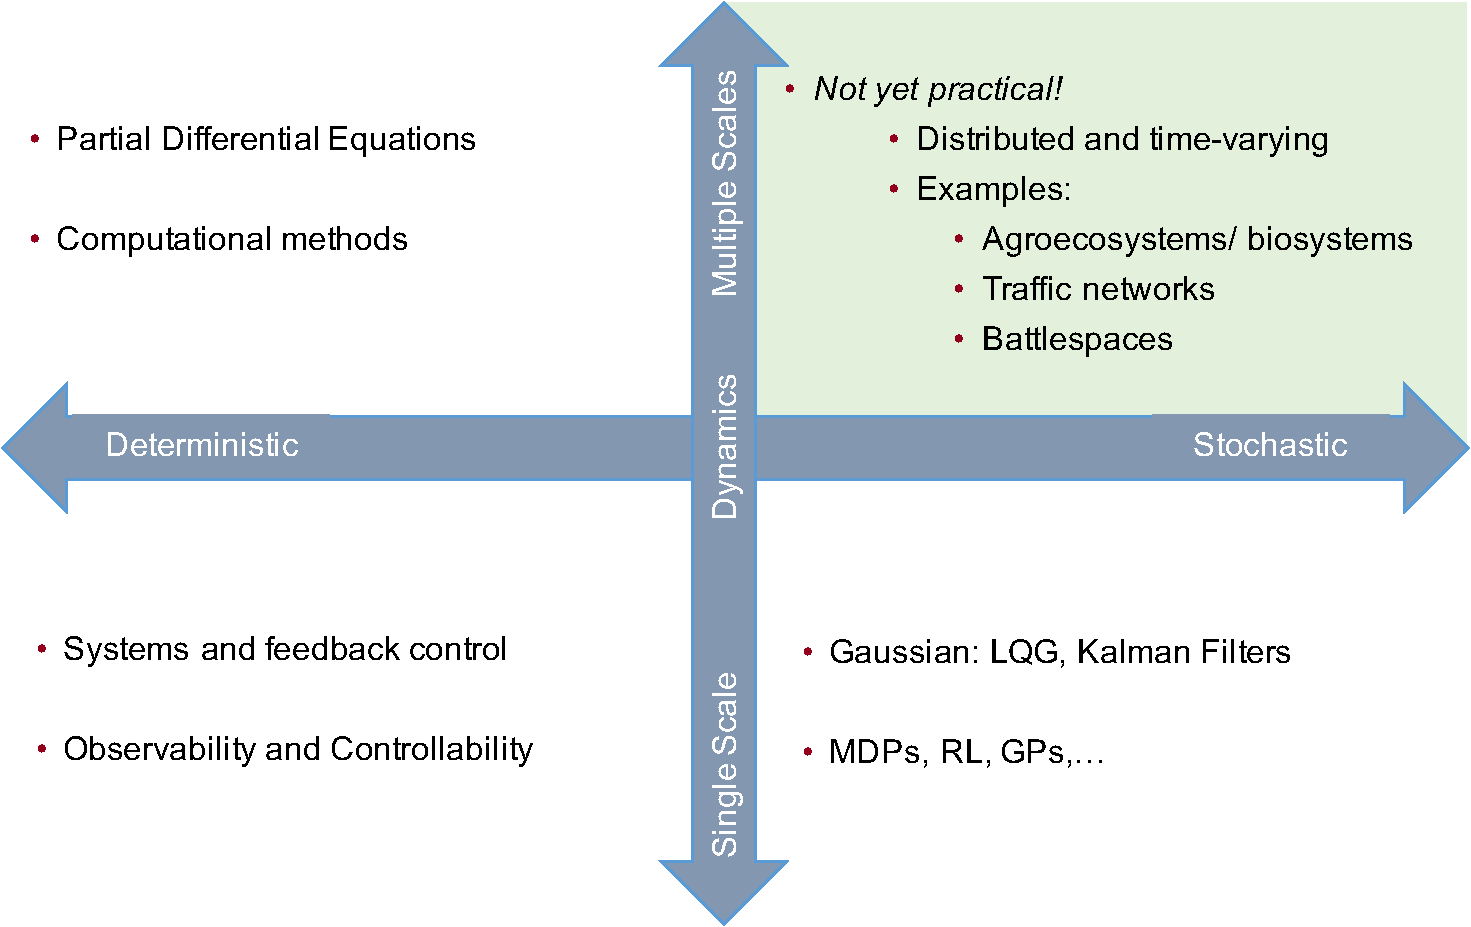
\includegraphics[width=\columnwidth]{CPS_SOA}
		\caption{Modeling, monitoring, and controlling dynamical systems with complex and uncertain dynamics, such as agricultural, traffic, or weather monitoring systems, presents exciting open challenge for the controls community. The bottom left quadrant describes linear and time-invariant systems with single- scale dynamics, for which the theory of feedback control of dynamical systems is often sufficient. The bottom right quadrant shows stochastic single-scaled systems, where approaches such as Kalman Filters and Gaussian optimization have marked several successes of control systems enabling endeavors from Lunar landings to GPS navigation. The top left quadrant denotes systems with dynamics at multiple scales, where efficient computational solutions to Partial Differential Equations (PDEs) is an highly active area of research. However, fundamental theoretical advances and practical algorithms are needed to enable autonomous decision making for distributed stochastic Cyber Physical Systems with dynamics at multiple scales – shown in the top right quadrant – such as distributed agricultural robotic systems, traffic networks, and weather monitoring systems with mobile and stationary sensors.}
	\label{fig:cps_soa}
\end{figure}
%Complex spatiotemporally varying systems such as agricultural systems, weather patterns, or fluid flows are typically difficult to address with traditional controls model with
  
Traditionally, the controls literature is strongest when the system dynamics can be represented as Ordinary Differential Equations (ODEs). % (see for example Figure \ref{fig:cps_soa}. Indeed %has focused on first principles and physics based models. As 
As depicted in Figure \ref{fig:cps_soa}, some of the major successes of controls have included results such as Linear Quadratic Gaussian control, reinforcement learning, and adaptive control in state spaces with well-defined, finite, and physically meaningful state variables. The problem of state estimation of a temporally evolving, finite-dimensional state-space system for example has been extensively studied in the context of Kalman filtering and observer design \cite{Gelb74}. Here, fundamental results in observability/controllability provide sufficient conditions on the structure of the state transition and measurement matrix such that the latent state can be estimated in the presence of measurement and process noise. %A highly successful example of such a state estimator is the celebrated Kalman filter, which is a Bayes-optimal filter for estimating the latent states of a finite-dimensional linear state-space model corrupted with Gaussian noise \cite{Gelb74}. 
On the other hand, machine learning models operate in an abstract and learned function-space of \textit{features} (for more details see ``\nameref{sb:featspace}''). Kalman filters can be naively extended to the functional domain (\cite{mardia1998kriged}), but have not typically been studied in context of the spatiotemporal monitoring problem studied here.  


On the other hand, recent advances in machine learning are providing different and highly powerful ways of modeling complex spatiotemporal dynamical systems.  %Yet %the sheer complexity of agricultural systems or weather patterns can make it difficult to design meaningful mo first principles based modeling highly limiting. Recent advances in machine learning would indicate that perhaps data-driven modeling could be very promising. 
Yet, the main challenge with using machine learning approaches such as deep learning or kernel based methods has been that these approaches lack interpretability and analyzability, which makes it difficult to design robust engineered systems. This is because machine learning works in abstract feature spaces that are only relatable to physical quantities through complex functional operations (see ``\nameref{sb:featspace}''). This leads to a major challenge in using machine learning models in control: For example, when kernel based models are used for spatiotemporal systems, how does one answer fundamental questions such as 1) the least number of sensors required to observe a distributed system, 2) the placement of sensors/actuators to guarantee observability/controllability of the system, and 3) the effect of random sensor placement on system observability/controllability.

In this paper we present an approach that can provide one formal way of addressing these and other questions about complex systems that are modeled with machine learning. In particular, we demonstrate how linear dynamical systems can be embedded in the reproducing kernel Hilbert space (RKHS) \cite{schoelkopf01kernelbased,ams:cucker,kingravi2012reproducing} generated by features used in Gaussian Process modeling \cite{Liu2018csmtutorial,rasmussen2006gaussian}, %machine learning feature spaces 
and utilized to answer fundamental questions such as controllability and observability. The marriage of systems theory with machine learning pursued in this paper is exciting, and % because it can provide a formal way of answering fundamental questions about complex systems, such as: % and seek to develop machine learning models that can be utilized to answer questions such as: 
 we expect that follow-up work will exploit the framework presented in this paper of utilizing linear models in RKHSs and feature spaces of other machine learning models to enable practical and analyzable data-driven engineering systems. To facilitate the development of the theory, we have focused this paper on the problem of monitoring spatiotemporal phenomena. However, the idea should be generalizable to any distributed cyber-physical system that is changing with space and time. %As such, we have focused mostly on the fundamental theory and practical algorithms in modeling, estimation, and control, while 
%The excruciating details of how to optimally implement the presented algorithms are omitted\footnote{Instead an open-source code-base is made available in MATLAB on http://daslab.illinois.edu/software.html and in Python on GitHub https://github.com/hkingravi/funcobspy?files=1}.   % that are analyzable.
\subsection*{Outline of the article and relationship to prior work by the authors}
 We begin the rest of the article by summarizing some related work in machine learning in this area.  ``\nameref{sb:featspace}'' discusses the concept of feature spaces and its importance in machine learning in a broader context. We then formulate the problem, introduce \emph{Kernel Observers (KO)}, and develop the main theoretical and algorithmic results.
This is followed by some results on the expected number of randomly placed sensors required to monitor a spatiotemporal process in the context of our model. An extension to the KO method called \emph{Evolving Gaussian Processes (E-GP)} is presented that learns one model for multiple, similar spatiotemporal processes, the efficacy of which on real-world CFD data is presented in Sidebar \emph{Learning Fluid Flows with Evolving Gaussian Processes}.
Elements of the work presented in this paper first appeared in Neural Information Processing Systems (NIPS 2016) (\cite{Kingravi16_NIPS,whitman2016NIPSworkshop}), IEEE CDC 2015 conference \cite{Kingravi:2015a}, the Conference on Robot Learning (CoRL 2017) \cite{whitman2017learning} and IEEE ACC 2018 conference \cite{Maske18_ACC}.  This paper presents a comprehensive set of results and fills in the missing links in a single encompassing publication, and introduces new results on observability in the presence of random sensor placement, and connections to Koopman operator theory. As such, we have focused in this article mostly on the fundamental theory and practical algorithms for modeling, estimation, and control, while the excruciating details of how to optimally implement the presented algorithms are omitted. Instead an open-source code-base is made available in MATLAB at \url{http://daslab.illinois.edu/software.html} or at \url{https://github.com/hkingravi/FunctionObservers} and in Python on GitHub at \url{https://github.com/hkingravi/funcobspy}.

%Section \ref{sec:exp} demonstrates the efficacy of the algorithms on several challenging and large real-world datasets.  and proofs of main results are provided in the Appendix. (IS THERE AN APPENDIX?)
